\documentclass{beamer}

% load packages
\usepackage[utf8]{inputenc}
\usepackage{graphicx}	% use graphic path
\usepackage{graphbox}	% needed to align graphics relative to text
%\usepackage[export]{adjustbox}
\usepackage{xcolor}		% needed for colored text
\usepackage{enumitem}	% use "plus" and "minus" symbols as bullets in itemize (pro/con lists)
\usepackage{tcolorbox} 	% draw a highlight box in the ICA slide

% setup enumitem in way compatible with beamer
\setitemize{label=\usebeamerfont*{itemize item}%
  \usebeamercolor[fg]{itemize item}
  \usebeamertemplate{itemize item}}

% set directory for the images
\graphicspath{{../images/}}

% setup theme
\usetheme{metropolis}

% title information
\title{Non-contact, automated cardiac pulse measurements using video imaging and blind source separation.}
\author{Ming-Zher Poh, Daniel J. McDuff, Rosalind W. Picard}
\date{2010}

\begin{document}

% own commands
\newcommand{\mytitle}[1]{{\Large{\underline{#1}}}}
\newcommand{\positiveaspect}{\textcolor{green}{$\oplus$}}
\newcommand{\negativeaspect}{\textcolor{red}{$\ominus$}}

% title page
\frame{\titlepage}

% start slides
\begin{frame}{Why to measure the pulse?}
\begin{itemize}
	\item General health indicator \pause
	\item Important for therapy of chronic diseases \pause
	\item Resting heart rate: risk factor of its own\\ \pause
		Comparable to smoking!\\
		
\includegraphics[width=1cm]{No_Smoking} \pause
	\item Scientific long term studies (e.~g. sleep studies)\\
		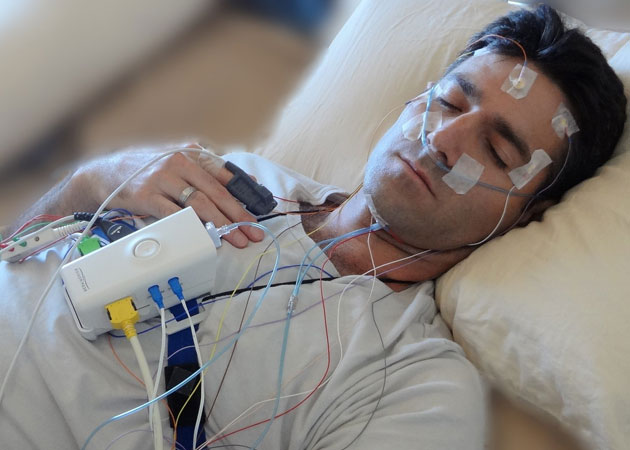
\includegraphics[width=0.4\textwidth]{Sleep-lab-facilities.jpg}
\end{itemize}
\end{frame}

\begin{frame}{Heart rate measurement (Traditional)}
\begin{itemize}
	\item \mytitle{Electrocardiography}\\
		\vspace{0.2cm}
		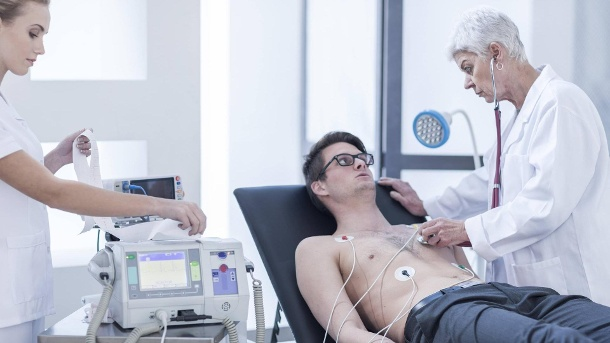
\includegraphics[width=0.45\textwidth, height=0.3\paperheight]{ekg.jpg}
		\hfill
		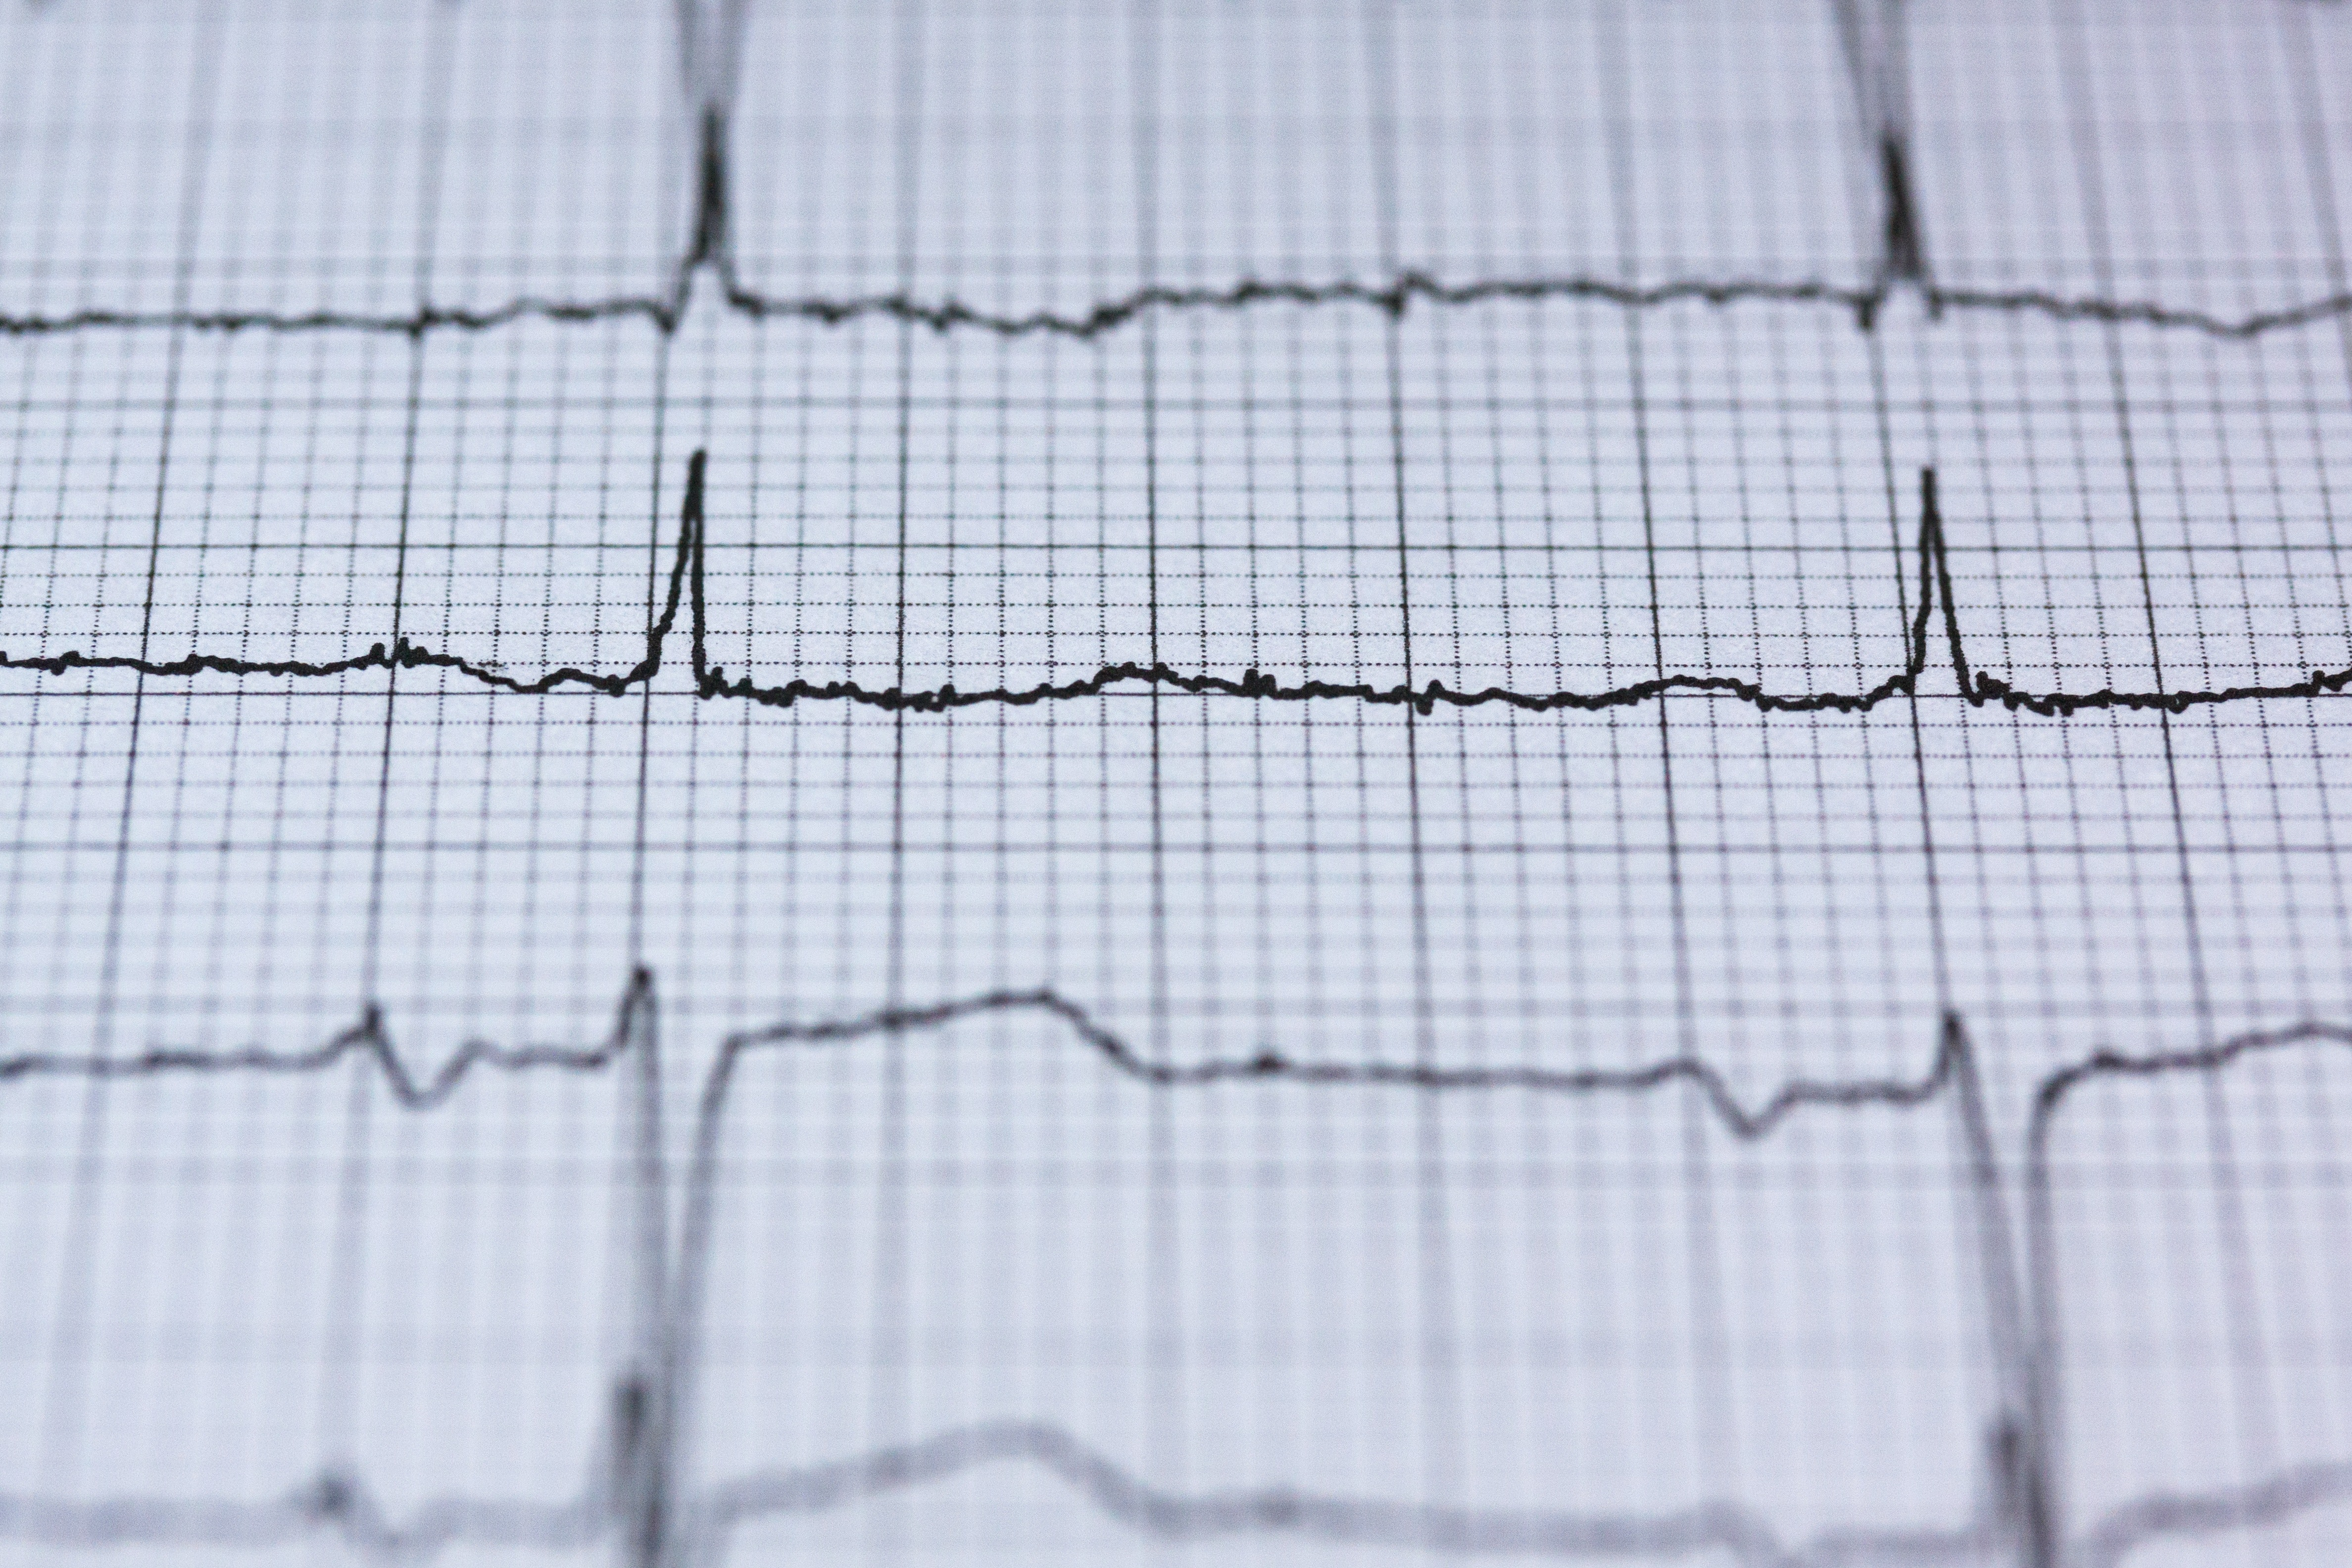
\includegraphics[width=0.45\textwidth, height=0.3\paperheight]{cardiogram.jpg}\\
		\noindent
		\begin{minipage}[t]{0.45\textwidth}
			\begin{itemize}[label=\positiveaspect]
				\item measure nerve impulse \pause
				\item very detailed, reliable \pause
				\item more than BPM \pause
			\end{itemize}
		\end{minipage}
		\hfill\vline\hfill
		\begin{minipage}[t]{0.45\textwidth}
			\begin{itemize}[label=\negativeaspect]
				\item cumbersome manual placement \pause
				\item usually in medical environment \pause
				\item uncomfortable
					
			\end{itemize}
		\end{minipage}
\end{itemize}
\end{frame}

\begin{frame}{Heart rate measurement (Traditional)}
	\begin{itemize}
		\item \mytitle{Photoplethysmography (PPT)}\\
			\vspace{0.2cm}
			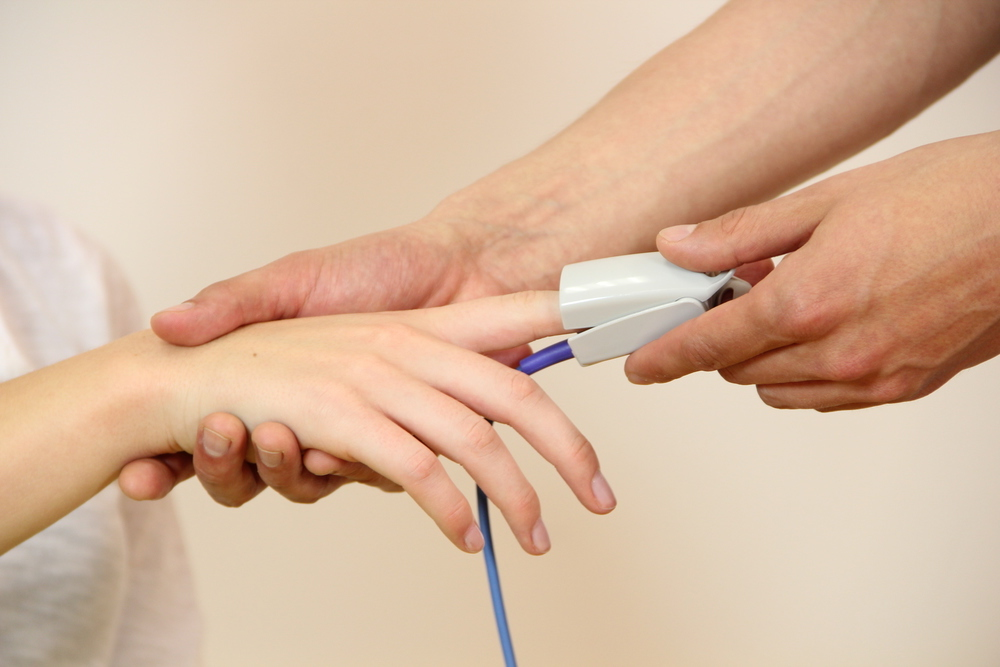
\includegraphics[width=0.45\textwidth, height=0.3\paperheight]{bvp_sensor_mirrored.jpg}
			\hfill
			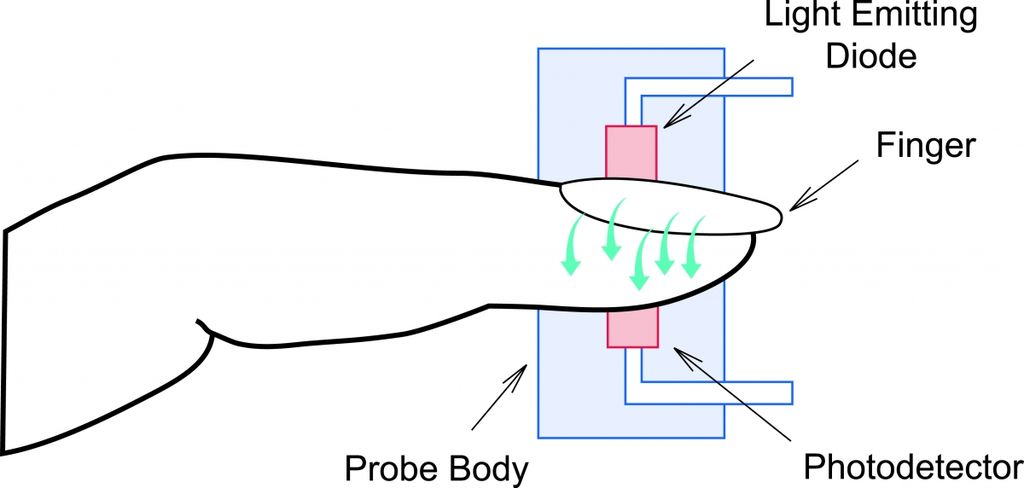
\includegraphics[width=0.45\textwidth, height=0.3\paperheight]{pulse_oximetry_sketch.jpg}\\ \pause
		\noindent
		\begin{minipage}[t]{0.45\textwidth}
			\begin{itemize}[label=\positiveaspect]
				\item fast \pause
				\item uncomplicated \pause
			\end{itemize}
		\end{minipage}
		\hfill\vline\hfill
		\begin{minipage}[t]{0.45\textwidth}
			\begin{itemize}[label=\negativeaspect]
				\item expensive (approx. 250~\$) \pause
				\item uncomfortable over long time
			\end{itemize}
		\end{minipage}
	\end{itemize}
\end{frame}

\begin{frame}{Traditional methods are reliable, but they...}
\pause
	\begin{itemize}[label=\negativeaspect]
		\item ... are expensive. \pause
		\item ... require medical personnel. \pause
		\item ... are uncomfortable for the patient. \pause
	\end{itemize}
	$\Rightarrow$ \textcolor{red}{\textbf{NOT SUITABLE}} for:\\
	\vspace{0.2cm} \pause
	\begin{minipage}[t]{\textwidth}
		\includegraphics[width=0.4\textwidth, align=c]{Sleep-Lab-facilities.jpg}
		\hspace{2cm}
		long time studies
	\end{minipage}\\ \pause
	\begin{minipage}[t]{\textwidth}
		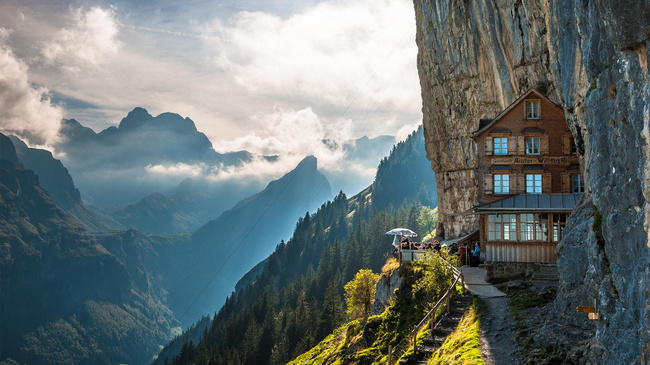
\includegraphics[width=0.4\textwidth, align=c]{berggasthaus_aescher.jpg}
		\hspace{2cm}
		telemedicine
	\end{minipage}
\end{frame}

\begin{frame}{A new hope: Using a camera}
	\begin{minipage}{0.3\textwidth}
		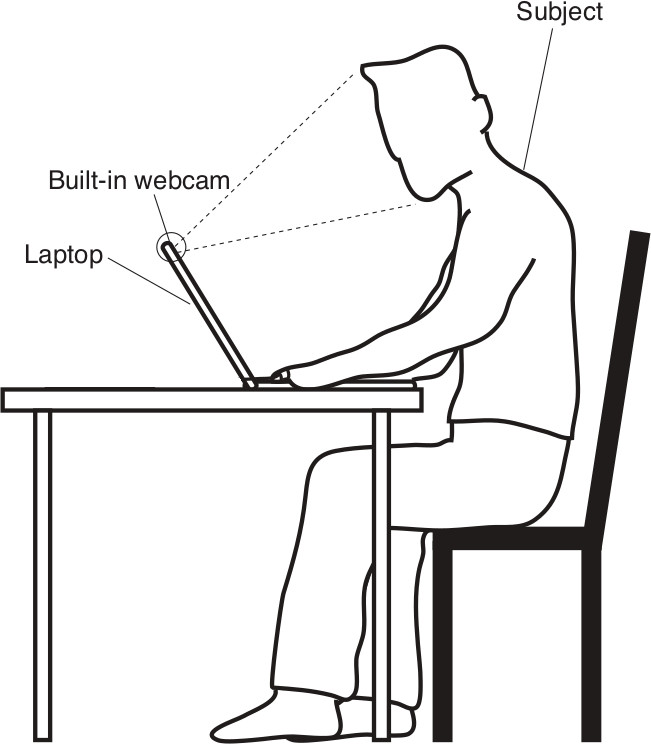
\includegraphics[width=\textwidth]{setup_no_bvp.jpg}
	\end{minipage} \pause
	\hfill
	\begin{minipage}{0.5\textwidth}
		\begin{itemize}[label=\positiveaspect]
			\item very cheap \pause
			\item everybody has a laptop/smartphone \pause
			\item very comfortable \pause
			\item can handle multiple patients at once
		\end{itemize}
	\end{minipage}
\end{frame}

\begin{frame}{Physical principle}
	\begin{itemize}
		\item \mytitle{Idea:}\\
			Absorption/reflection depends on thickness of blood vessels\\
			\begin{center}
				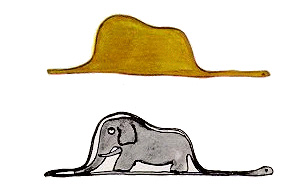
\includegraphics[width=0.5\textwidth]{snake.jpg}
			\end{center} \pause
		\item Reflected light from face depends on cardiac cycle \\ \pause
			$\Rightarrow$ Measurable using a camera! \pause
		\item Problem: \textbf{\textcolor{red}{NOISE!}} \pause
		\item Solution: \textbf{\textcolor{green}{Independent Component Analysis (ICA)}}
	\end{itemize}
\end{frame}

\begin{frame}{Independent Component Analysis (ICA)}
	\begin{itemize}
		\item Detects underlying "true" signals in a measured signal\\
			(blind source separation) \pause
		\item \underline{Assumed model:}
			\begin{center}
			\tcbox{$\vec{x} = A \cdot \vec{s}$,}
			\end{center} \pause
			\begin{itemize}
				\item $\vec{x} = \begin{pmatrix}
					x_1 \\
					\vdots \\
					x_n
				\end{pmatrix}$ measured (mixed) signal \pause
				\item $\vec{s} = \begin{pmatrix}
					s_1 \\
					\vdots \\
					s_n
				\end{pmatrix}$ latent pure signal ("true signal") \pause
				\item $x_1, \dots, x_n$ \textbf{\textcolor{red}{NOT INDEPENDENT}}\\
					$s_1, \dots, s_n$ \textbf{\textcolor{green}{INDEPENDENT}} \pause
				\item ICA computes $W \approx A^{-1}$
			\end{itemize}
	\end{itemize}
\end{frame}

\begin{frame}{ICA vs. PCA}
	\begin{itemize}
		\item Conceptually similar to PCA \pause
		\item \textbf{PCA assumption:}\\
			most information in vectors with biggest variance\\ \pause
			\textbf{ICA assumption:}\\
			most information in vectors that are independent \pause
	\end{itemize}
	$\Rightarrow$ ICs correspond to physical phenomena: \textbf{\textcolor{green}{INTERPRETABLE}}!
\end{frame}

\begin{frame}{ICA: Calculation and Problems}
	\begin{itemize}
		\item \mytitle{Calculation}
			\begin{itemize}[label=-]
				\item Basic idea: Use Central Limit Theorem \pause
				\item Linear combinations of true signals are "more Gaussian" than the true signals themselves\\ \pause
					$\Rightarrow$ Obtain ICs by maximizing "Non-Gaussianity" \pause
			\end{itemize}
		\item \mytitle{Problems} \pause
			\begin{itemize}[label=\negativeaspect]
				\item No natural order of ICs \pause
				\item Not clear how many ICs to assume (heuristics exist)
			\end{itemize}
	\end{itemize}
\end{frame}

\begin{frame}{Algorithm}
\textbf{\Large 1.) Face detection} (in each frame)\\
	\vspace{0.2cm}
	\begin{minipage}{\textwidth}
	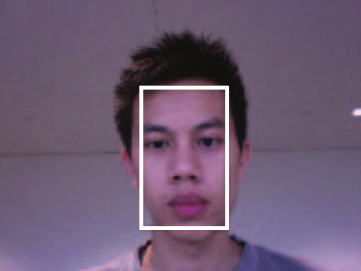
\includegraphics[width=0.5\textwidth, align=c]{face_detection.png} \pause
	\hfill
	
\includegraphics[width=0.3\textwidth, align=c]{OpenCV_Logo.png} \pause
	\end{minipage}\\
	\vspace{0.5cm}
	Pretrained Viola-Jones model provided by OpenCV\\ \pause
	\vspace{0.5cm}
	$\Rightarrow$ Region of interest (ROI)
\end{frame}

\begin{frame}{Algorithm}
\textbf{\Large 2.) Obtaining the mixed signals} (in each frame)
	Spatial average over ROI in each colour channel
	\begin{figure}
	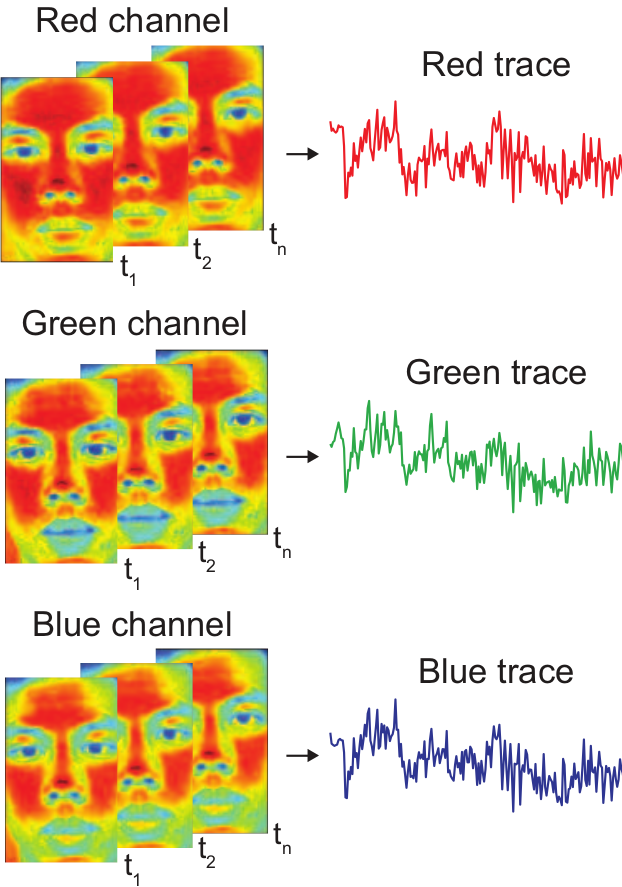
\includegraphics[height=0.6\paperheight, align=c]{video_to_trace.png}
	\end{figure}
	$\Rightarrow x_1(t), x_2(t), x_3(t)$
\end{frame}

\begin{frame}{Algorithm}
\textbf{\Large 3.) Normalise}
\begin{itemize}
	\item Within a moving 30~s - window:\\
		Calculate $\mu_i, \sigma_i$ \pause
	\item Normalise:
		\begin{equation*}
			x'_i = \frac{x_i(t) - \mu_i}{\sigma_i}, i = 1, 2, 3
		\end{equation*}
\end{itemize}
\end{frame}

\begin{frame}{Algorithm}
\textbf{\Large 4.) Get independent true signals}
\begin{figure}
	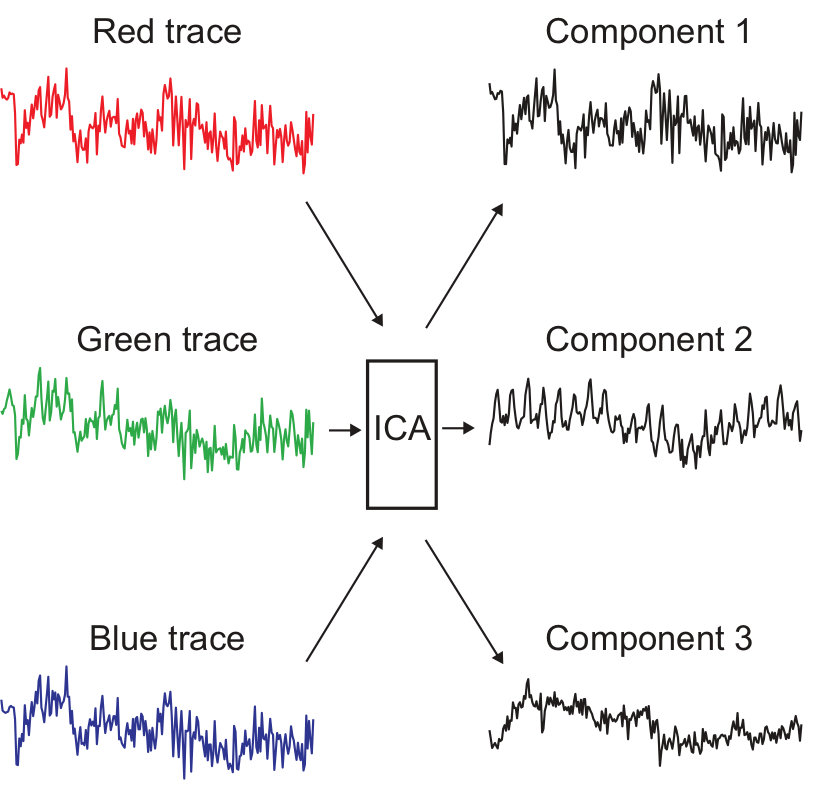
\includegraphics[width=0.5\textwidth]{paper_ica.png}
\end{figure}
\end{frame}

\begin{frame}{Algorithm}
\textbf{\Large 5.) Obtain heart rate}
\begin{itemize}
	\item Apply FFT to get power spectrum:
		\begin{figure}
			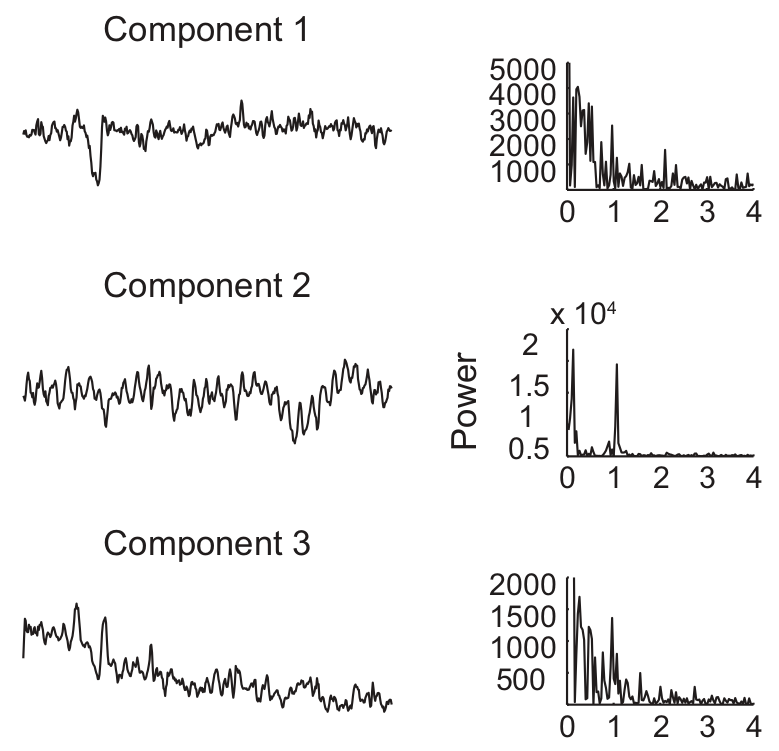
\includegraphics[height=0.3\paperheight]{paper_power_spectrum.png}
		\end{figure}
	\item Select highest power peak of the spectrum
	\item Include constraints: Heart rate must ...
		\begin{itemize}[label=-]
			\item ... be in range [45, 240]~bpm
			\item ... not change more than 12~bpm within 1~s
		\end{itemize}
\end{itemize}
\end{frame}

\end{document}